\chapter{Analysis Software}

The analysis of vdM data, along with the application of stability and linearity corrections, is carried out using two distinct frameworks, each playing a crucial role in ensuring the accuracy and reliability of the results.

The vdM Framework \cite{VdMFramework} is employed to execute all the corrections and fits detailed in \autoref{ch:2023_luminosity_calibration}. This tool is vital for managing the complex data processing required during the vdM scans, enabling precise calibration and adjustment of the luminometers. My contributions to the development and enhancement of this framework are discussed in \autoref{sec:the_vdM_framework}.

For integration corrections, the BRIL work suite (b' database. To query this database, and obtain the corrected datarilws) \cite{xie_bril} is utilized. This suite takes on the critical task of applying the final layer of luminosity corrections, as well as distributing the results to other CMS groups. The specific program responsible for these corrections is called brilcalc. The inner workings, limitations, developed alternatives, and my contributions to the improvement of this program are detailed in \autoref{sec:the_bril_work_suite}.

\section{The vdM Framework}
\label{sec:the_vdM_framework}

The vdM Framework (vdMFw) is the analysis software used by CMS to perform luminosity calibration measurements for all luminometers with per-bunch granularity. First commissioned in 2015, it has been continuously improved in line with the collaboration’s growing understanding of the systematics discussed in \autoref{ch:2023_luminosity_calibration}. Today, it serves as the primary framework for analyzing vdM scans, applying data corrections, and tracking luminometer operational conditions through emittance scan analysis throughout the year.

\subsection{Flow of the Analysis}

The flow of analysis in the vdMFw, outlined in \autoref{fig:vdm_fw_flowchart}, begins with user-provided input. This input can be categorized into two types: the data to be analyzed and the user specifications that dictate how the analysis should be conducted.

\begin{figure}[!htb]
	\centering
	\makebox[\textwidth]{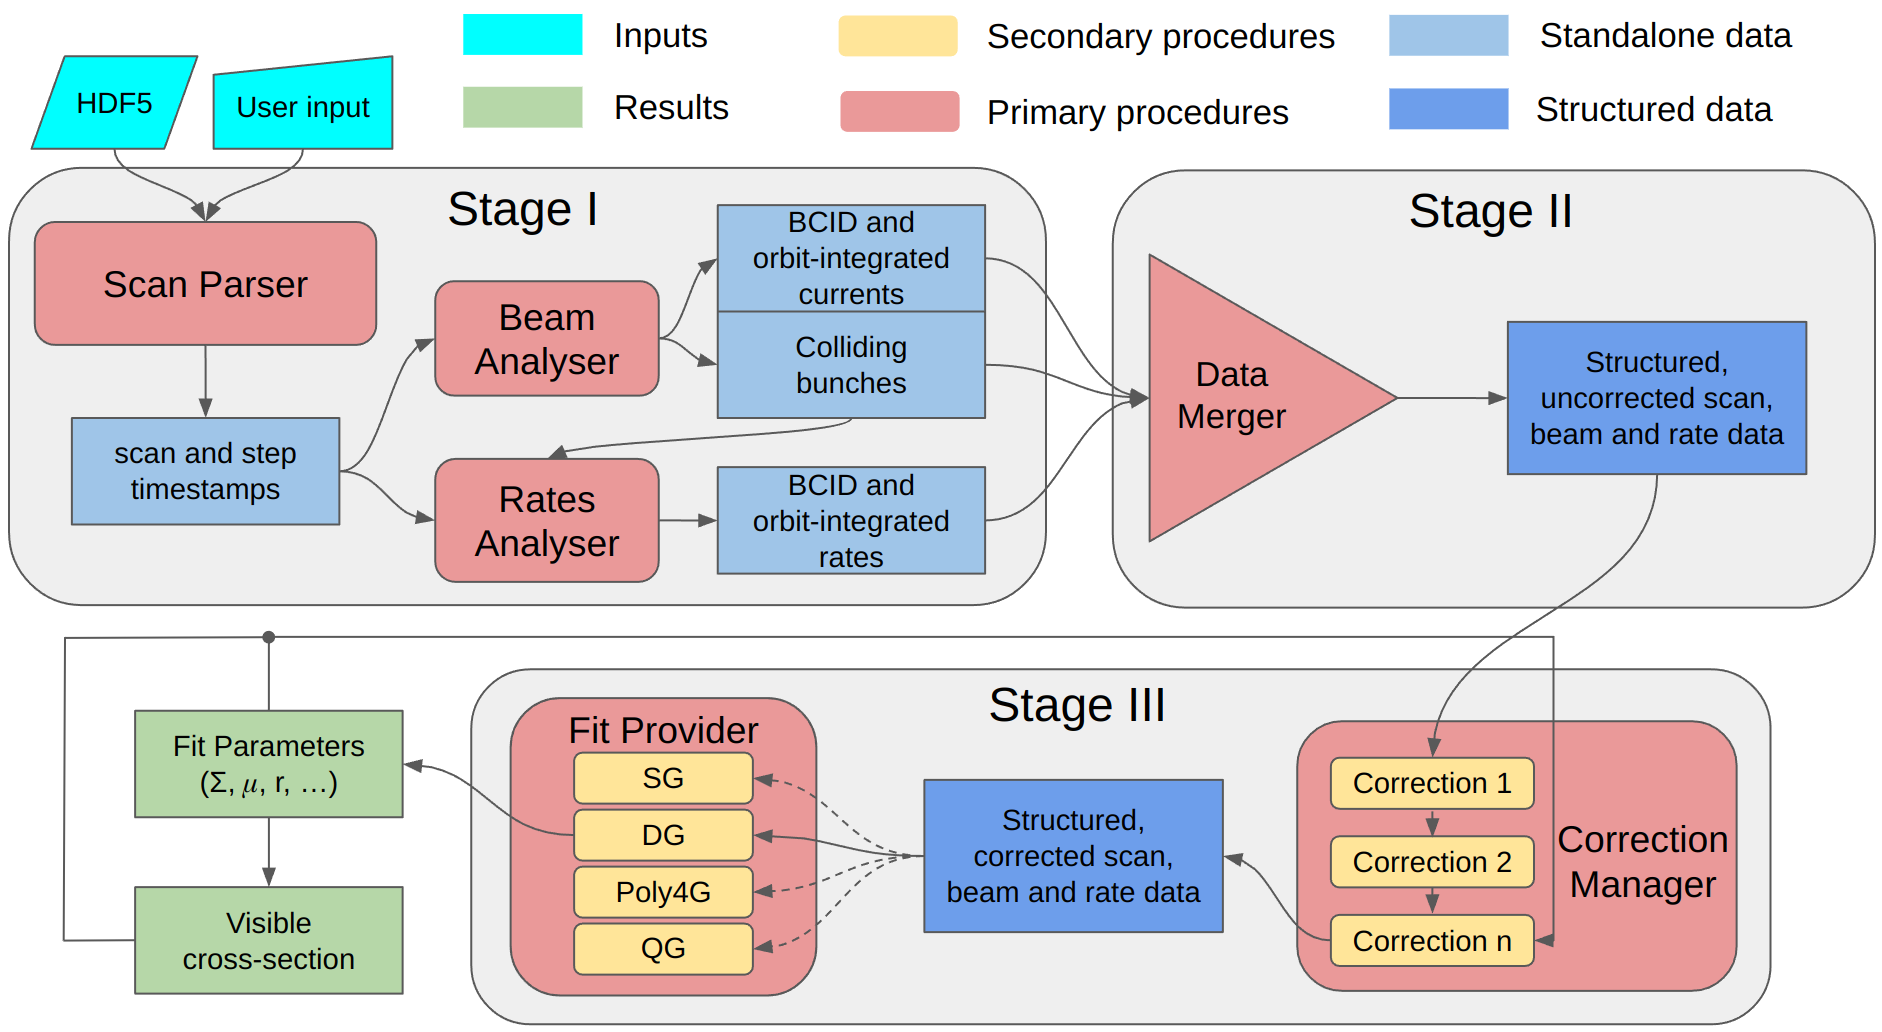
\includegraphics[width=0.7\paperwidth]{images/assets/vdm_fw_flowchart.png}}
	\caption{Overview of the flow of the analysis in the vdMFw.}
	\label{fig:vdm_fw_flowchart}
\end{figure}

The data is provided in Hierarchical Data Format 5 (HDF5) \cite{koranne2011hierarchical}, which includes scan, luminometer, and beam information for a particular period of time:
\begin{itemize}
	\item \textbf{Scan data}: Includes beam separation information, which is used to extract the beginning and end timestamps of each scan step.
	\item \textbf{Beam data}: Contains the beam currents, both per-orbit and per-bunch, saved in the beam table of the input file.
	\item \textbf{Luminometer data}: Stores the counts for every luminometer in operation during the time period associated with the input file.
\end{itemize}
The user can specify the following input parameters:
\begin{itemize}
	\item Which luminometer data to analyse. The results of the analysis will correspond to the calibration constant for this luminometer.
	\item The fit function to be used for the bunch overlap shapes.
	\item The corrections to be applied. Some corrections are derived from the input data file, while others require external inputs from parallel analyses.
	\item Optionally, the user may provide a \textit{ratefile}, also in HDF5 format, which contains only luminometer rates. This is useful when the original luminometer data is corrupted, non-existent, or when some offline correction has been applied to the original data.
\end{itemize}
Additionally, there is a user configuration file where further details can be adjusted.

The first stage of the analysis involves the preparation of the individual inputs that go into the fitting procedure, such as the beam separations and the rates normalized to the beam currents. The Scan Parser extracts the timestamps associated with each scan step and feeds them into the subsequent blocks. The Beam Analyser identifies the colliding bunches and computes the beam currents. At this stage, the beam current corrections explained in \autoref{subsec:beam_current_measurement} are applied. The colliding bunch indices are then passed to the Rates Analyser, where the luminometer rates are calculated.

The data processed in the previous stage is passed to Stage II. This stage consolidates all the pieces of information into a structured format to facilitate the application of any corrections and fits that follow.

Lastly, Stage III applies all the requested corrective procedures, and finishes in a fit to the corrected data, which provides the fit parameters used in calculating the detector calibration constants. While all corrections are done sequentially, some require outputs from previous corrections, hence the backward connector from the results to the beginning of this stage. The analysis concludes with all the results, both intermediate and final, being saved to files for later inspection.

\subsection{Input/Output bottleneck}
\label{subsec:io_bottleneck}

The vdMFw is executed multiple times throughout the year, particularly during emittance scans and vdM fills, where numerous corrections must be applied. Additionally, the process of adjusting the calibrations and ensuring detector stability is highly iterative, requiring the analysis to be run repeatedly until the results achieve the desired precision. Consequently, efforts have been made to enhance the software's performance.

To identify the primary bottlenecks within the framework, an initial profiling was conducted on input HDF5 files corresponding to vdM scans. These files were chosen because they undergo the complete correction pipeline, providing a comprehensive diagnosis of performance issues.

The profiling was performed on a system with the following specifications: x86\_64 architecture, equipped with 32 CPUs, each with 2 threads per core, distributed across 8 cores per socket, and 2 sockets in total. The CPUs operate at a base frequency of 1.0 GHz, with a maximum frequency of 3.5 GHz, supported by 64 GB of RAM and an L3 cache of 11 MB.

The results of the profiling are presented in \autoref{tab:profiling_results}, which highlights the time spent in each stage of the analysis process.

\begin{table}[!htb]
	\centering
	\caption[Initial vdMFw profiling results]{Initial profiling results shown separately for the procedures in Stage I and combined for Stages II and III. The times correspond to an average of 50 runs where the full analysis pipeline was executed.}
	\begin{tabular}{|l|c|c|}
		\hline
		\textbf{Procedure} & \textbf{Time [s]} & \textbf{\% of total program} \\
		\hline
		Scan Parser        & 0.34 $\pm$ 0.01   & 0.27                         \\
		Beam Analyser      & 37.11 $\pm$ 0.65  & 29.60                        \\
		Rate Analyser      & 57.85 $\pm$ 1.18  & 46.15                        \\
		Stage II + III     & 30.06 $\pm$ 0.57  & 23.98                        \\
		\hline
	\end{tabular}
	\label{tab:profiling_results}
\end{table}

As shown in \autoref{tab:profiling_results}, the most significant bottlenecks were identified in the Beam Analyser and Rate Analyser procedures, which together account for over 75\% of the total execution time. This result was unexpected, as the bulk of the framework’s workload was anticipated to revolve around data corrections and fitting procedures.

Upon closer inspection of the code within these two time-consuming procedures, the reason for their substantial execution time became apparent. To generate the expected outputs, these procedures need to read relevant data from the input HDF5 files. In the original implementation, the reading process occurred for every scan step, as follows:

\begin{enumerate}
	\item Read the entire rate (or beam) table\footnote{HDF5 files are organized in folder-like structures. The \textit{tables} are analogous to files in this structure, and in BRIL's case, each table contains specific data related to the LHC.} from the HDF5 file into memory.
	\item Filter for the timestamps corresponding to the current scan step.
\end{enumerate}

Reading the entire table content each time is computationally expensive, as the amount of data to be read can consume a significant portion of the execution time. The profiling mentioned above was conducted using data files already filtered by the time period during which the scan was performed, resulting in smaller data files (approximately 23 MB). However, when the same profiling was run with an optional \textit{ratefile} of 1631 MB in memory, the execution time of the Rate Analyser procedure increased dramatically from 57.85 seconds to 446.34 seconds, clearly indicating an Input/Output-related bottleneck.

To improve these execution times, the following optimizations were implemented:

\begin{itemize}
	\item The corresponding rate (or beam) table is now read only once before computing the per-step results.
	\item Instead of loading the entire table content into memory, which could lead to crashes if the data size exceeds the available RAM + SWAP\footnote{SWAP space is a portion of the hard drive designated to act as virtual memory when the physical RAM is fully utilized. It helps prevent crashes by providing additional memory space, though it is much slower than actual RAM.} space, a first pass is performed to gather all the entries that fall within any scan step.
	\item Only the relevant entries identified in the previous step are then read.
\end{itemize}

These changes led to the improved profiling results shown in \autoref{tab:profiling_results_2}:

\begin{table}[!htb]
	\centering
	\caption[vdMfw profiling results after performance improvements]{Profiling results after implementing the optimizations in the analyser procedures. The results show significant improvements in both procedures. The bulk of the framework (Stages II and III) now accounts for 95\% of the total program execution time, and the overall program speedup was approximately 4 times.}
	\begin{tabular}{|l|c|c|}
		\hline
		\textbf{Procedure} & \textbf{Time [s]} & \textbf{\% of total program} \\
		\hline
		Scan Parser        & 0.35 $\pm$ 0.02   & 1.08                         \\
		Beam Analyser      & 0.90 $\pm$ 0.11   & 2.80                         \\
		Rate Analyser      & 0.36 $\pm$ 0.02   & 1.11                         \\
		Stage II + III     & 30.46 $\pm$ 0.54  & 95.01                        \\
		\hline
	\end{tabular}
	\label{tab:profiling_results_2}
\end{table}

When running the profiling on the same larger \textit{ratefile} as before, the average execution time was reduced to $7.9 \pm 0.22$ seconds, representing a speedup of approximately 56 times compared to the original implementation.

\subsection{Online vdM Analysis}

An important aspect of analyzing LHC scans is the ability to process data immediately after a scan is completed, a process referred to as online analysis. Quick feedback from the framework allows for the possibility of repeating scans if any issues are identified during their execution. This capability is especially critical during vdM fills, motivating the enhancements made to this workflow.

\begin{figure}[!htb]
	\centering
	\makebox[\textwidth]{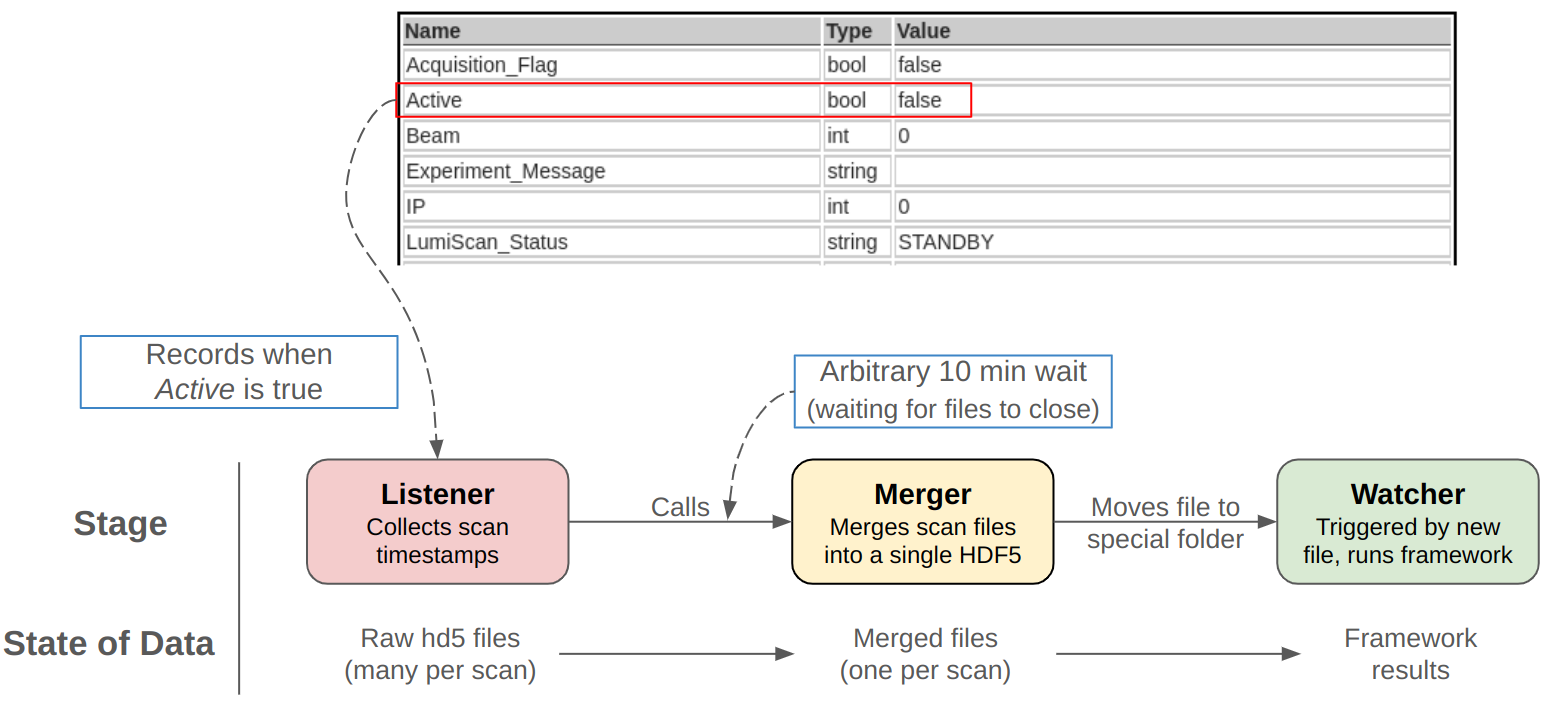
\includegraphics[width=0.7\paperwidth]{images/assets/online_analysis_workflow.png}}
	\caption{Workflow of the online analysis.}
	\label{fig:online_analysis_workflow}
\end{figure}

The workflow, illustrated in \autoref{fig:online_analysis_workflow}, begins with the Listener stage. This component constantly queries the xDAQ data acquisition system \cite{Brigljevic:845273} for the \textit{Active} variable, which is set to true while a scan is ongoing at the CMS IP. During these periods, two independent processes are at work:

\begin{itemize}
	\item \textbf{BRIL Data Acquisition System (BRILDAQ)}: BRILDAQ, built on top of xDAQ, is the data transfer system used by all BRIL systems. It is configured to save extra HDF5 files to a specific destination while \textit{Active} is set to true. These files are smaller and each contains data for a portion of the entire scan.
	\item \textbf{Scan Listener}: The Listener, a separate process also built using xDAQ, continuously monitors the \textit{Active} variable and records the timestamps corresponding to the beginning and end of a scan (when \textit{Active} changes from false to true and from true to false).
\end{itemize}

Once a scan is completed, the Listener passes the timestamp information to the Merger, which consolidates all files created within those timestamps. Since the two processes mentioned earlier operate independently, a safeguard in the form of a 10-minute wait time was implemented to protect against potential I/O errors. The output of the Merger is a single file containing data for the entire scan. This file is then moved to a designated folder monitored by the Watcher.

The Watcher is a filesystem event manager designed to trigger whenever a new file is created in a specific directory. Each trigger initiates the vdMFw to analyze that particular scan, applying multiple fits, corrections, and processing all online luminometers.

\subsection{Improving Wait Time in Merger}

The fixed waiting time in the Merger block is suboptimal. If the wait time is too short, it could lead to I/O problems, whereas if it is too long, it could delay the ability to repeat a scan, which is particularly critical during vdM fills.

To address this, an alternative approach was introduced in the Merger step that continuously polls the intermediate HDF5 files to check if they have been closed. This was implemented using the \textit{lsof} Linux utility, which provides a convenient API to determine which files are open by which processes. The implementation of this polling mechanism can be seen in \autoref{lst:merger_polling}.

During the 2024 vdM program, which started on May 16th, the time spent waiting for the files to close for all vdM and im scans was significantly shorter than the fixed 10-minute interval, as shown in \autoref{tab:time_waiting_2024}.

\begin{table}[!htb]
	\centering
	\caption{Time spent waiting for scan files to close in the Merger during the 2024 vdM fill.}
	\begin{tabular}{|c|c|c|c|c|c|c|c|c|}
		\hline
		\textbf{Scan}     & vdm1  & vdm2  & vdm3  & vdm4  & vdm5  & im1   & im2   & vdm6  \\
		\hline
		\textbf{Time [s]} & 27.97 & 24.53 & 25.04 & 26.69 & 32.79 & 18.29 & 19.19 & 27.25 \\
		\hline
	\end{tabular}
	\label{tab:time_waiting_2024}
\end{table}

Being the most time consuming stages of this workflow the wait time in the Merger and running the vdMFw, these improvements allow for a feedback time of approximately 1 min after a particular scan has finished, a significant improvement over the 10+ minutes it used to take previously.
 

\section{The BRIL Work Suite}
\label{sec:the_bril_work_suite}

The \textit{brilcalc} tool, part of the BRIL work suite, plays a critical role in providing other CMS groups with access to the most accurate and up-to-date luminosity data from BRIL. This section will first explain how \textit{brilcalc} operates, including the necessary special input files, before discussing the enhancements made to its usability and maintenance. Finally, a highly requested alternative to \textit{brilcalc} will be introduced, along with an analysis of its advantages and disadvantages.

\subsection{Normtags and Iovtags}

\begin{figure}[!htb]
	\centering
	\makebox[\textwidth]{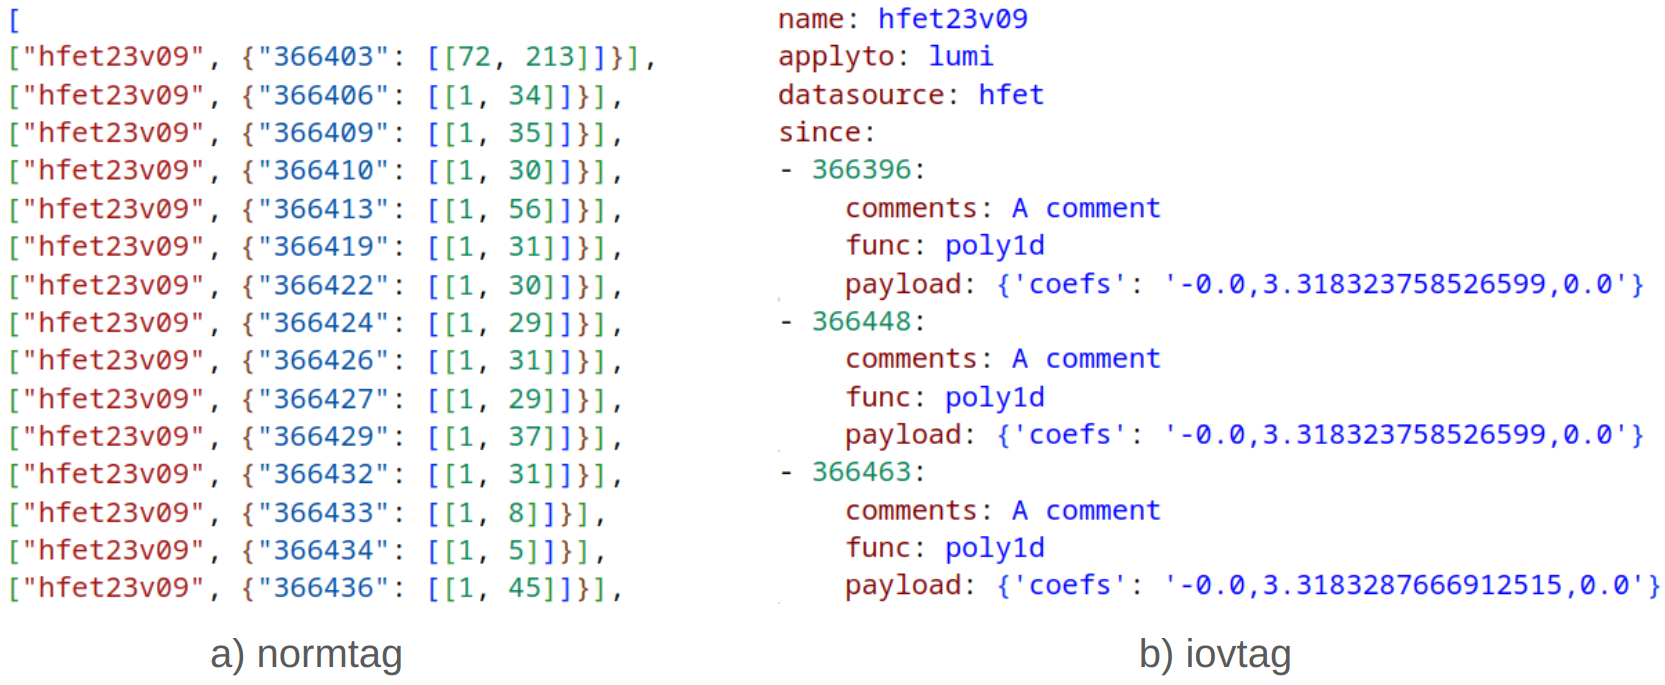
\includegraphics[width=0.7\paperwidth]{images/assets/normtag_iovtag.png}}
	\caption[Illustration of iovtag and normtag file structure]{a) Example of a Normtag file specifying LHC periods for queries in brilws' database. Each period is defined by a run number and a range of valid lumisections for that run. b) Example of an Iovtag file corresponding to the HFET luminometer, specifying correction functions and payload arguments for each run number at the beginning of a fill.}
	\label{fig:normtag_iovtag}
\end{figure}

Given the high data demands from both BRIL and other CMS groups, \textit{brilcalc} needs to efficiently retrieve luminosity results for any requested period. To meet this requirement, data initially stored in HDF5 files is loaded into the brilws database. \textit{Brilcalc} relies on two specific input files for querying the database: a \textit{normtag} and an \textit{iovtag} file. The \textit{normtag} file defines the LHC periods to be queried, while the \textit{iovtag} file specifies how to apply corrections to the data from those periods. The structure of these files is illustrated in \autoref{fig:normtag_iovtag}.

To interpret these files:
\begin{itemize}
	\item The first entry in the normtag specifies: For all lumisections in $[72, 213]$ of run 366403, use the iovtag hfet23v09.
	\item The first entry in the iovtag specifies: For all runs in $[366396, 366447]$, correct HFET's luminosity by applying the function \textit{poly1d} with the parameters \textit{\{'coefs': '-0.0,3.318323758526599,0.0'\}}.
\end{itemize}

The correction applied by the \textit{poly1d} function corresponds to the procedure explained in \autoref{subsec:extrapolation_of_vdM_calibration}. The \textit{coefs} field contains three comma-separated values that represent the coefficients of a second-degree polynomial in descending order. Since \textit{brilcalc} operates on rate data from the HDF5 files, the coefficients are derived using:

\begin{equation}
    \centering
    \mathcal{L} = \underbrace{C_0}_{\text{0th order}} + \underbrace{\frac{f_{rev}}{\sigma_{vis} \cdot \epsilon}}_{\text{1st order}} \mu + \underbrace{- \alpha \left( \frac{f_{rev}}{\sigma_{vis} \cdot \epsilon} \right)^{2}}_{\text{2nd order}} \mu^2
    \label{eq:brilcalc_poly1d}
\end{equation}

\subsection{Limitations}

Despite being the primary tool for obtaining the latest luminosity results, \textit{brilcalc} was not originally designed for iterative analysis processes. Each time a new version of HDF5 data for a specific luminometer is created, it must be uploaded to the database. This process is not only time-consuming, as only authorized maintainers can update the database, but it also poses a risk of contaminating the database with incorrect data since uploads are not automatically validated for accuracy.

There are also issues with the construction of iovtags. As shown in \autoref{fig:normtag_iovtag}b, the \textit{payload} parameter of iovtags is often not descriptive, requiring creators to add meaningful comments that help users interpret the values of $\sigma_{\text{vis}}$, $\epsilon$, and $\alpha$ that generated the \textit{coefs}.

Another significant problem is the lack of thorough validation for iovtags submitted to the database. The original system only checks the iovtag schema, not its content. Combined with minimal commenting, this can complicate the management of multiple iovtags across different systems and increase the difficulty of ensuring reproducibility of results.

\subsection{Enhancements to Iovtags}

The software responsible for applying corrections specified by \textit{iovtags} is built around a Python class containing various methods for implementing different types of luminosity corrections. For each correction, the specific method to be called is determined by the \textit{func} parameter within the \textit{iovtag}, and the method uses the corresponding \textit{payload} to compute the corrected luminosity. Below is a simplified version of the existing code:

\begin{lstlisting}
class LuminosityCorrector:
  def poly1d(self, database_input, payload):
    coefs_array = np.fromstring(payload["coefs"], dtype=np.float, sep=',')

    # Logic to fetch the rates and number of colliding bunches from the database
    rates = ...
    ncol = ...

    # Divide by ncol to get the SBIL
    return ncol * np.poly1d(rates / ncol, coefs_array[::-1])
\end{lstlisting}

The first enhancement to the iovtag workflow was to introduce a new set of payload parameters. A new function, \textit{poly1d2}, where "2" denotes version 2, was implemented as follows:

\begin{lstlisting}
def poly1d2(self, database_input, payload):
  # Logic to fetch the rates and number of colliding bunches from the database
  rates = ...
  ncol = ...

  lumi = (payload["frev"] * rates / ncol) / (payload["sigvis"] * payload["eff"])
  return payload["constant"] + lumi - payload["alpha"] * lumi**2
\end{lstlisting}

This alternative implementation provides several advantages:

% \begin{itemize}
%     \item When using \textit{poly1d2}, the payload values become transparent, allowing anyone with access to the \textit{iovtag} to see the individual components rather than just the final coefficients from \autoref{eq:brilcalc_poly1d}. This is demonstrated in the following example:

% 	\begin{lstlisting}[language=Yaml]
% - 366396:
%   comments: A comment
%   func: poly1d2
%   payload:
%     frev: 11245.5
%     sigvis: 3394.33
%     eff: 1.02
%     slope: 0.0
%     constant: 0.0
% 	\end{lstlisting}

%     \item The new format simplifies comparisons between different versions of \textit{iovtags} for the same system, as only the \textit{comments} and \textit{payload} values differ. In the previous format, users could only guess what caused differences in coefficients.

%     \item The payload arguments effectively document the \textit{iovtag}, reducing the reliance on comments, which can often be incorrect or outdated. This self-documentation increases the robustness of \textit{iovtags} over time, as the essential details are embedded within the parameters themselves.

%     \item Including the calculation components directly within the \textit{iovtag} centralizes the code, reducing the risk of errors when applying the formula described in \autoref{eq:brilcalc_poly1d}.
% \end{itemize}

This alternative implementation offers several advantages. Firstly, when using \textit{poly1d2}, the payload values become transparent, allowing anyone with access to the \textit{iovtag} to see the individual components rather than just the final coefficients from \autoref{eq:brilcalc_poly1d}. This is evident in the following example:

\begin{lstlisting}[language=Yaml]
- 366396:
    comments: A comment
    func: poly1d2
    payload:
        frev: 11245.5
        sigvis: 3394.33
        eff: 1.02
        slope: 0.0
        constant: 0.0
\end{lstlisting}

This new format simplifies comparisons between different versions of \textit{iovtags} for the same system, as only the \textit{comments} and \textit{payload} values differ, whereas in the previous format, users could only speculate about the reasons behind differences in coefficients. Moreover, the payload arguments effectively document the \textit{iovtag}, reducing reliance on comments, which can often be incorrect or outdated. This self-documentation makes \textit{iovtags} more robust over time, embedding essential details directly within the parameters themselves. Additionally, including the calculation components directly within the \textit{iovtag} centralizes the code, reducing the risk of errors when applying the formula described in \autoref{eq:brilcalc_poly1d}.

Although this new approach improves the readability of \textit{iovtags}, it does not fully address the lack of stable, up-to-date documentation for the parameters of each method within the corrector class, nor does it validate \textit{iovtags} upon upload. To address both issues while maintaining tight coupling with the source code, Python decorators were employed \cite{pep318}.

A decorator named \textit{register\_sanitizer} was used on all correction methods to document each \textit{payload} parameter. An example of decorating the \textit{poly1d2} method is shown below:

\begin{lstlisting}
@register_sanitizer(
  required_params=(
    ("frev", "LHC's revolution frequency."),
    ("sigvis", "Luminometer visible cross-section."),
    ("eff", "Efficiency factor applied to 'sigvis'."),
    ("alpha", "Slope extracted from a linear fit to sbil_1 / sbil_2 = a * sbil_2 + b."),
    ("constant", "0th degree coefficient of the 2nd-degree polynomial."),
  )
)
def poly1d2(self, database_input, payload):
  ...
\end{lstlisting}

This decorator ensures that the \textit{poly1d2} function checks for the presence of all required parameters in the \textit{iovtag} before executing. For methods requiring constraints on parameters, the decorator also accepts a \textit{validators} parameter, as shown below:

\begin{lstlisting}
@register_sanitizer(
  required_params=(
    ("frev", "LHC's revolution frequency."),
    ("sigvis", "Luminometer visible cross-section."),
    ("eff", "Efficiency factor applied to 'sigvis'."),
    ("alpha", "Slope extracted from a linear fit to sbil_1 / sbil_2 = a * sbil_2 + b."),
    ("intercept", "Intercept extracted from the linear fit."),
    ("constant", "0th degree coefficient of the 2nd-degree polynomial."),
  ),
  validators=(
    (lambda payload: not np.isclose(payload["alpha"], 0.0), "'alpha' parameter cannot be 0."),
  )
)
def another_method(self, database_input, payload):
  ...
\end{lstlisting}

In the implementation of this decorator (see \autoref{lst:register_sanitizer}), the attributes \textit{\_required\_params} and \textit{\_validators} are added to the function objects to differentiate them from other class attributes. A class decorator named \textit{collect\_sanitizers} is used as a metaclass \cite{pep3115}, which gathers all registered sanitizers into class attributes upon loading, as illustrated in \autoref{lst:collect_sanitizers}.

This setup allows the sanitizers to be used not only on already loaded iovtags but also on those requested for upload. The \textit{validate\_iovtag\_data} function, shown in \autoref{lst:validate_iovtag_data}, implements the validation logic and is called each time a new iovtag is to be uploaded.

All these modifications allow the users of brilws to be more certain of the contents of the \textit{iovtags} they use as well as prevents poluting the database with erroneous correctors.


% \subsection{An alternative to brilcalc}

% The most theckincally challenging aspect of luminosity analysis is managing the different data versions. Any experimental effect that was not dealt with during operations has to be corrected for in offline analysis in a process that is tipically reffered to as reprocessing. Every reprocessing, takes as input a particular version of the HDf5 data for a given system, or systems, and corrects for one or multiple systematics. The result, is a new set of HDF5 files with the added correction.

% In principle, every new set of HDF5 files would be checked to assert that the correction was correctly applied. However, the checking of the results often required that the files were first uploaded to brilws' database. This, apart from leading to potential polution of the data in the database, leads to an extra data version in the database. An alternative, capable of producing the same outputs as brilcalc from just HDF5 files, was hightly requested.

% The software solution, although separate from brilws, was developed to be compatible to brilws workflow. It asks users to provide a \textit{nomrtag} file as well as the path location of the HDF5 files to be corrected. The \textit{iovtags} refered in the \textit{nomrtag} have to exist in disk but do not need to be loaded onto any database. The final output of this tool is in the same as in brilcalc. This tool opens up the possibility to rigorously test the result of any reprocessing before deciding to share the data with the rest of CMS.

% Even though the output of both tools is the same, there are advantages to using each:

% \begin{itemize}
% 	\item This alternative leaves no doubt has to what version of the data is being analysed since a path to the datafiles must be provided.
% 	\item The alternative is considerably slower then the brilws implementation. This is because reading the data directly from disk is considerably slower than querying a database.
% 	\item Even though its slower, it is fast enough as to allow multiple iterations of the analysis. In fact, for 2023 the stability and non-linearity corrections for the BCM1F system benifited mostly from it as multiple versions of this analysis took place. 
% \end{itemize}

% In conclusion, this alternative is extremely usefull for doing actual analysis while brilcalc is now used as the production equivalent for the analysis results. 

\subsection{An Alternative to brilcalc}

One of the most technically challenging aspects of luminosity analysis is managing the different versions of data. Any experimental effect not addressed during operations must be corrected in offline analysis, a process commonly referred to as reprocessing. Each reprocessing step takes as input a specific version of the HDF5 data for a given system or set of systems and applies corrections for one or more systematic effects, resulting in a new set of HDF5 files with the added corrections.

Ideally, each new set of HDF5 files would be thoroughly checked to ensure that the corrections were properly applied. However, verifying the results often required that the files first be uploaded to the brilws database, which not only risked contaminating the database with incorrect data but also unnecessarily increased the number of data versions stored. Consequently, there was a high demand for an alternative tool capable of producing the same outputs as \textit{brilcalc} directly from HDF5 files without the need for database integration.

The proposed software solution, while separate from brilws, was designed to be compatible with the brilws workflow. It requires users to provide a \textit{normtag} file and specify the location of the HDF5 files to be analyzed. The \textit{iovtags} referenced in the \textit{normtag} must exist on disk but do not need to be loaded into any database. The final output of this tool matches the format produced by \textit{brilcalc}, enabling rigorous testing of any reprocessing results before deciding to share the data with the rest of the CMS.

Although both tools produce the same output, each has distinct advantages. The alternative tool provides absolute certainty regarding the version of the data being analyzed since users must specify the exact path to the data files. However, this alternative is significantly slower than the brilws implementation because reading data directly from disk is much slower than querying a database. Despite this slower speed, it is still fast enough to allow multiple iterations of analysis, making it particularly useful for 2023, where the stability and non-linearity corrections for the BCM1F system benefited greatly from this approach, as multiple reprocessing steps were required.

In conclusion, while this alternative tool proves invaluable for conducting detailed analyses, \textit{brilcalc} remains the preferred option for production-level results, offering a more streamlined and faster approach once the data is finalized.
